\section{Auswertung}
\label{sec:Auswertung}

Für den Strom aus der einfallenden Intensität wurden $I_e = \SI{0,54}{\milli\ampere}$ gemessen. Die Messdaten für parallel polarisiertes Licht sind in
\autoref{tab:ppolMess}, die Daten für senkrecht polarisiertes Licht in \autoref{tab:spolMess} eingetragen. Der Brechungsindex für senkrecht und parallel
polarisiertes Licht wurde durch umstellen der jeweiligen Fresnel'schen Formel \eqref{eqn:fresnelsenk} und \eqref{eqn:fresnelpara} berechnet. Die Werte sind ebenfalls in den beiden Tabellen eingetragen.
Für die Energie $E$ wurde der Wert $\sqrt{\sfrac{I_r}{I_e}}$ eingesetzt.
\newpage


\begin{table}[H]
    \centering
    \caption{Messdaten mit dem sich daraus ergebenden Brechungsindex bei parallel polarisiertem Licht.}
    \label{tab:ppolMess}
    \begin{tabular}{c c c}
        \toprule
        Winkel in Grad & Photostrom / $\si{\micro\ampere}$  & Brechungsindex $n:\parallel$ \\
        \midrule
        10.0  &  4.7  &  3.903  \\
        12.0  &  4.4  &  4.226  \\
        14.0  &  3.8  &  28.04  \\
        16.0  &  3.1  &  4.264  \\
        18.0  &  2.9  &  6.544  \\
        20.0  &  2.2  &  11.134  \\
        22.0  &  2.1  &  4.759  \\
        24.0  &  1.6  &  11.698  \\
        26.0  &  1.2  &  7.973  \\
        28.0  &  0.9  &  5.555  \\
        30.0  &  0.8  &  35.852  \\
        32.0  &  0.9  &  6.843  \\
        34.0  &  0.8  &  6.93  \\
        36.0  &  0.8  &  47.267  \\
        38.0  &  0.75  &  6.503  \\
        40.0  &  0.7  &  9.551  \\
        44.0  &  0.5  &  6.677  \\
        48.0  &  0.44  &  10.886  \\
        50.0  &  0.42  &  7.369  \\
        52.0  &  0.45  &  44.481  \\
        54.0  &  0.41  &  8.907  \\
        56.0  &  0.39  &  8.814  \\
        58.0  &  0.37  &  64.206  \\
        60.0  &  0.35  &  8.17  \\
        62.0  &  0.35  &  11.743  \\
        64.0  &  0.36  &  20.504  \\
        66.0  &  0.35  &  8.161  \\
        68.0  &  0.33  &  18.811  \\
        70.0  &  0.3  &  13.262  \\
        72.0  &  0.3  &  8.806  \\
        74.0  &  0.28  &  50.281  \\
        76.0  &  0.25  &  10.613  \\
        78.0  &  0.22  &  10.332  \\
        80.0  &  0.22  &  81.3  \\
        82.0  &  0.25  &  9.567  \\
        84.0  &  0.42  &  13.522  \\
        86.0  &  0.83  &  24.251  \\
        88.0  &  0.52  &  9.417  \\
        \bottomrule
    \end{tabular}
\end{table}
\newpage

\begin{table}[H]
    \centering
    \caption{Messdaten mit dem sich daraus ergebenden Brechungsindex bei senkrecht polarisiertem Licht.}
    \label{tab:spolMess}
    \begin{tabular}{c c c}
        \toprule
        Winkel in Grad & Photostrom / $\si{\micro\ampere}$  & Brechungsindex $n_\perp$ \\
        \midrule
        10.0  &  4.7  &  0.964  \\
        12.0  &  4.4  &  0.985  \\
        14.0  &  3.8  &  1.001  \\
        16.0  &  3.1  &  1.018  \\
        18.0  &  2.9  &  1.043  \\
        20.0  &  2.2  &  1.061  \\
        22.0  &  2.1  &  1.092  \\
        24.0  &  1.6  &  1.117  \\
        26.0  &  1.2  &  1.144  \\
        28.0  &  0.9  &  1.176  \\
        30.0  &  0.8  &  1.215  \\
        32.0  &  0.9  &  1.263  \\
        34.0  &  0.8  &  1.308  \\
        36.0  &  0.8  &  1.361  \\
        38.0  &  0.75  &  1.415  \\
        40.0  &  0.7  &  1.474  \\
        44.0  &  0.5  &  1.605  \\
        48.0  &  0.44  &  1.767  \\
        50.0  &  0.42  &  1.861  \\
        52.0  &  0.45  &  1.969  \\
        54.0  &  0.41  &  2.084  \\
        56.0  &  0.39  &  2.215  \\
        58.0  &  0.37  &  2.363  \\
        60.0  &  0.35  &  2.53  \\
        62.0  &  0.35  &  2.724  \\
        64.0  &  0.36  &  2.949  \\
        66.0  &  0.35  &  3.211  \\
        68.0  &  0.33  &  3.52  \\
        70.0  &  0.3  &  3.891  \\
        72.0  &  0.3  &  4.349  \\
        74.0  &  0.28  &  4.92  \\
        76.0  &  0.25  &  5.655  \\
        78.0  &  0.22  &  6.636  \\
        80.0  &  0.22  &  8.018  \\
        82.0  &  0.25  &  10.101  \\
        84.0  &  0.42  &  13.614  \\
        86.0  &  0.83  &  20.704  \\
        88.0  &  0.52  &  41.543  \\
        \bottomrule
    \end{tabular}
\end{table}


\noindent
Die aus den Brechungsindizes berechneten Mittelwerte lauten
\begin{align*}
    \overline{n_\parallel} &=  4.391 \pm 7.259 \ , \\
    \overline{n_\perp} &= 1,041 \pm 0,037.
\end{align*}


\begin{figure}[H]
    \centering
    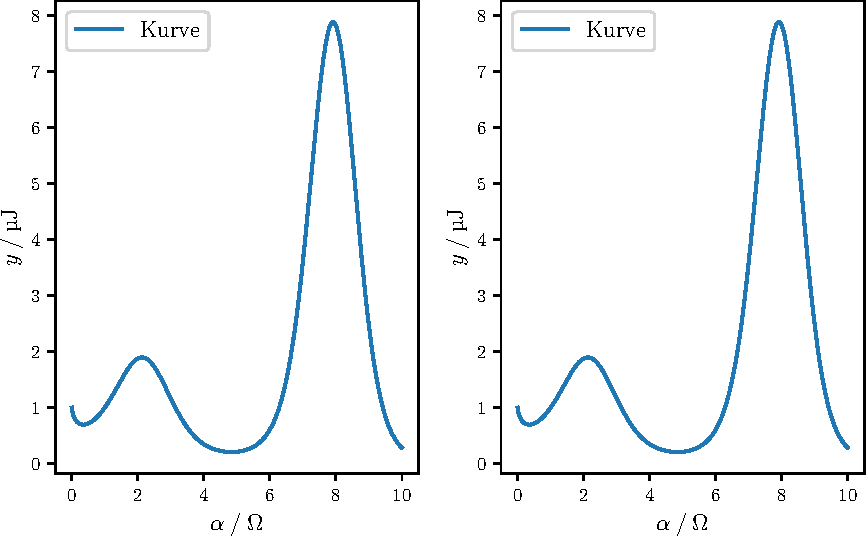
\includegraphics[width=\textwidth]{build/plot.pdf}
    \caption{Grafische Auswertung der Messdaten mit den jeweiligen Theoriekurven.}
    \label{fig:plot}
\end{figure}

\noindent
In \autoref{fig:plot} wurden die Messdaten mit den jeweiligen Theoriekurven grafisch dargestellt. Für die Theoriekurven wurde in die Gleichungen \eqref{eqn:fresnelsenk} und \eqref{eqn:fresnelpara}
ein Literaturwert von
\begin{align*}
    n_{\text{Lit}} = 3,353
\end{align*}
eingesetzt \cite{BrechSilizium}. Die grafische Auswertung liefert näherungsweise einen Brewsterwinkel von  
\begin{align*}
    \alpha_{\text B} = \SI{78}{\degree},
\end{align*}
und daraus ein Brechungsindex von 
\begin{align*}
    \tan(\alpha_{\text B} = \SI{78}{\degree}) = 4,705.
\end{align*}